% Setup - do not change
\documentclass[11pt]{article}
\usepackage[top=0.9in, left=0.9in, bottom=0.9in, right=0.9in]{geometry} 
\usepackage{parskip}

\usepackage[english]{babel}
\usepackage[utf8]{inputenc}
\usepackage{amsmath,amsthm,amssymb,graphicx,pdfpages,lipsum,hyperref}
\usepackage[none]{hyphenat}
\usepackage{csquotes}
\usepackage{float}
\setlength\parindent{0pt}
%%%%%%%%%%%%%%%%%%%%%%%%%%%%%%%%%%%%%%%%%%%%%%%%%%%%%%%%%%%%%%%%%%%
% add other packages here if required

%% Bibliography are specified in this file. You can also choose inline bib style if you want to. But make sure your citation style is consistent (and proper)
% For more details on citation: https://library.unimelb.edu.au/recite
\usepackage[sorting = none]{biblatex}
\addbibresource{references.bib}

%%%%%%%%%%%%%%%%%%%%%%%%%%%%%%%%%%%%%%%%%%%%%%%%%%%%%%%%%%%%%%%%%%% the '%' symbol denotes comments

% Begin document creation
% DELETE THE \lipsum PLACEHOLDERS WHEN YOU BEGIN
\title{\textbf{Factors Affecting the Use of Yellow Taxis in NYC \\ A Survey between Late 2021 and Early 2022}}
 
\author{
Jiajia Guo \\
Student ID: 1135319 \\
%% Replace the link with your github repo
% 1. Remember to escape underscore (\_) in the link.
% 2. Remember to include the commit you want to submit in the link
%\href{https://github.com/MAST30034-Applied-Data-Science/mast30034\_p1\_template/tree/fd9f1dd17fdbcb5b119b70c93a22da8210d44fd7}{Github repo with commit}
}
https://github.com/MAST30034-Applied-Data-Science/mast30034-project-1-arya9uo/commit/10e6bce4e47688765b0b5ab5b9273ec2cbe76b97


\begin{document}
\maketitle

\section{Introduction}
% Link to a 30 min tutorial if you require revision: https://www.overleaf.com/learn/latex/Learn_LaTeX_in_30_minutes
Traditionally, yellow taxis have served as an icon of New York City (NYC) \cite{medallion}. They are allowed to pick up passengers anywhere in NYC. In contrast, green taxis serve areas outside of central Manhattan \cite{diff}. Before the outbreak of Covid-19 in 2020, a constant stream of yellow taxis is very common in Manhattan. 
However, before the lockdown in 2020, yellow taxis were already underwater due to the rapid growth of ride-hailing apps like Uber and Lyft. On August 8th, 2018, NYC became the first American city to allow ride-hailing vehicles to operate on its roads legally \cite{uber}. Passengers who are fed up with unreliable and dirty taxi ride migrate to ride-hailing apps which promise cleaner rides and friendly drivers.

Apart from the increased competition from Uber and other apps, yellow taxi drivers owed \$600,000 medallion debt on average to pay for their license operating on the roads \cite{medallion}. 

Being a yellow taxi driver was a path to middle-class life for lower-class citizens or newly arrived immigrants. Not only the drivers but also citizens and local government are managing to save this iconic city transportation. 

In this report, we survey between November 2021 and February 2022 about the factors affecting the use of yellow taxis after NYC reopening in June 2021. In November 2021, NYC was nearly fully reopening except for schools. In January 2022, the omicron variant sends NYC. Covid-19 case numbers soaring to records \cite{hit}. The doubled infections caused public panic and put pressure on transportation. 


The goal of our report is to answer questions about the factors that influence the use of yellow taxis:
\begin{itemize}
\item After reopening, will a new peak in Covid-19 infections affect the use of yellow taxis?
\item With the increased price of riding-hailing, is it still more attractive than yellow taxis for riders?
\item Do passengers have different tipping behaviors towards riding-hailing and yellow taxis?
\item How to build a machine learning model to forecast the tip amounts and how to measure the model performance?
\end{itemize}

 
\section{Data}
We aim to investigate the influence of Uber usage frequency on yellow taxis after reopening. Therefore, we collect trip records of yellow taxi and HVFHS (high volume for-hire services)  between Nov 2021 and Feb 2022 from the New York City Taxi and Limousine Commission (TLC) \footnote{https://www1.nyc.gov/assets/tlc/downloads/pdf/trip\_record\_user\_guide.pdf}. To figure out whether the outbreak of Covid-19 variants still has a huge impact on the yellow taxi trips or not, We collected the cumulative counts of coronavirus cases in the United States from The New York Times between November 2021 and February 2022. \footnote{https://github.com/nytimes/covid-19-data}.

\subsection{Data Preprocessing}
\subsubsection{Yellow Taxi}

\paragraph{Data Cleaning}
\begin{itemize}
     \item 4\% of instances contain NaN values. Impute NaN values with the most frequent value in each column.
    \item Filter rate to standard rate and JFK rate as they are relevant to analysis and account for almost all instances in the data sets. Approximately 93\% riders are charged with standard rate, 3\% riders are charged with JFK rate.
    \item Filter payment method to credit card and cash as they are two most popular payment methods. Approximately 77\% riders choose to pay with credit card, 22\% of them pay with cash.
    \item Remove Store\_and\_fwd\_flag column as it was not relevant to analysis.
\end{itemize}



The upper figures in Figure \ref{fig:explore_yellow} show the outliers in five numerical attributes in the yellow taxi dataset. The figures below in Figure \ref{fig:explore_yellow} show the value distribution from these five attributes after removing outliers. The following are the steps of outlier removal.
\paragraph{Outlier Removing}
\begin{itemize}
    \item Remove instances where pick-up time are later than or equal to drop-off times.
    \item Remove instances where total amounts do not vary between 0 and \$250.
    \item Remove instances where fare amounts do not vary between 0 and \$180.
    \item Remove instances where tip amounts do not vary between 0 and \$180.
    \item Remove instances where trip time do not vary between 0 and 80000 seconds.
    \item Remove instances where trip distances do not vary between 0 and 400 miles.
\end{itemize}

\begin{figure}
    \centering
    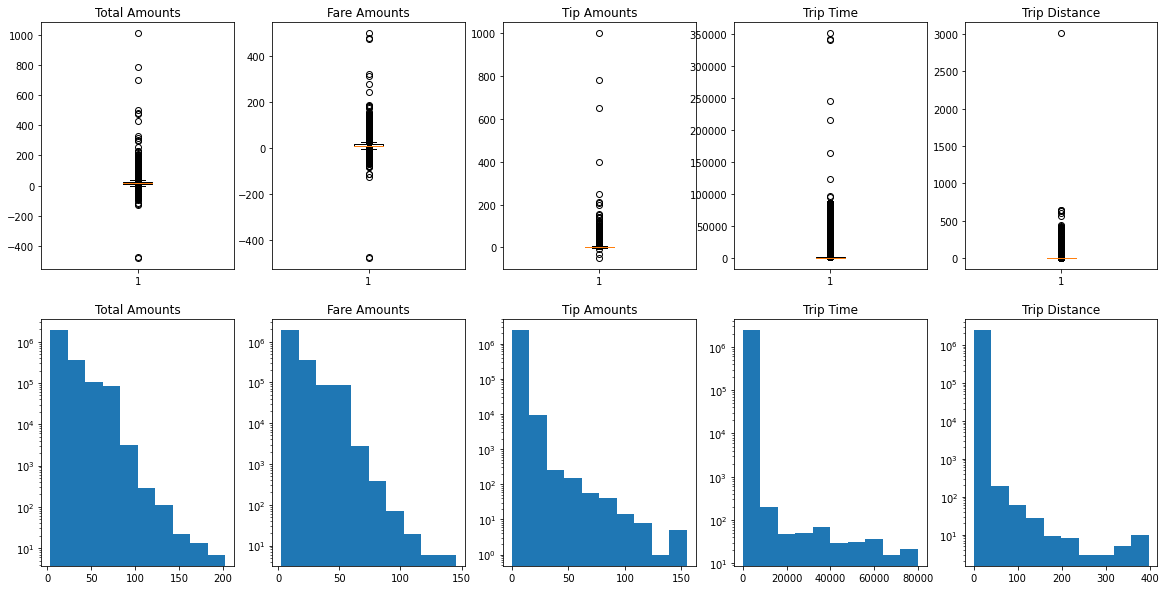
\includegraphics[scale = 0.38]{explore_yellow.png}
    \caption{The upper figures are the box plots of total amounts (\$), fare amounts (\$), tip amounts (\$), trip time (Second) and trip distance (Mile). The separate circles are outliers. The figures below are histograms of those five attributes after removing outliers. The data comes from yellow taxi dataset in Nov 2021.}
    \label{fig:explore_yellow}
\end{figure}

\subsubsection{High Volume For-Hire Services Data (HVFHS)}
Because Uber is the largest ridesharing company in the United States, we concentrate on Uber among other alternatives for analysis. 

\paragraph{Data Cleaning}
\begin{itemize}
    \item 30 \% of instances contain NaN values. Impute NaN values with the most frequent value in each column.
    \item Filter riding-hailing service to just Uber.
    \item Drop columns Dispatching\_base\_num and Originating\_base\_num as they are irrelevant to our analysis.
    \item Drop columns Request\_datetime and On\_scene\_datetime as we keep Pickup\_datetime	Dropoff\_datetime that also occurs in yellow taxi data.
    \item Drop columns related to flags such as the mentioned services are rarely used.
\end{itemize}
\paragraph{Outlier Removing}
\begin{itemize}
    \item  Remove instances where pick-up time are later than or equal to drop-off times.
    \item Remove instances where fare amounts do not vary between 0 and \$600 .
    \item Remove instances where tip amounts do not vary between 0 and \$100.
    \item Remove instances where trip time do not vary between 0 and 25000 seconds.
    \item Remove instances where trip distances do not vary between 0 and 120 miles.
\end{itemize}

\begin{figure}
    \centering
    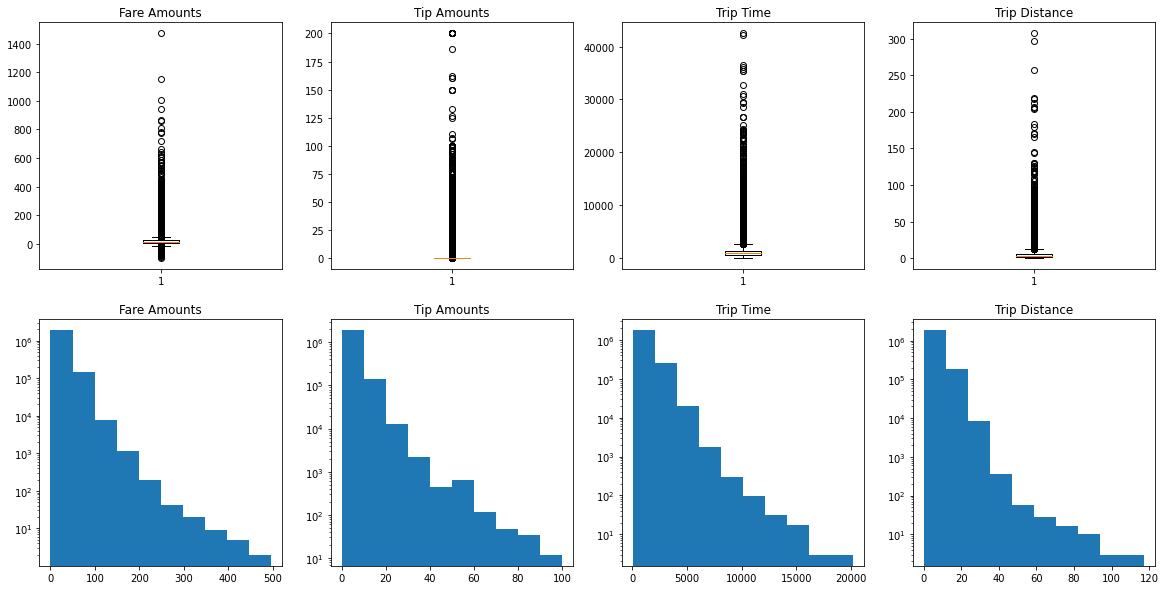
\includegraphics[scale = 0.35]{explore_fhvhv.png}
    \caption{The upper figures are the box plots of fare amounts (\$), tip amounts (\$) , trip time (Second) and trip distance (Mile). The separate circles are outliers. The figures below are histograms of those four attributes after removing outliers. The data comes from HVFHS dataset in Nov 2021.}
    \label{fig:explore_fh}
\end{figure}
\subsubsection{Covid-19 Data}
We focus on NYC and remove instances related to other cities or states. To better observe whether there exists a peak of Covid-19 infections, the amount of daily new confirmed cases is determined by calculating the difference between the daily total confirmed cases in the current row and that in the previous row. 


%On March 24th 2022, Uber announces its cooperation with yellow taxis in NYC. It means that on the Uber app, passengers will find Yellow taxis as their driving options. 

\subsection{Analysis}
\subsubsection{Covid-19}
\begin{figure}
    \centering
    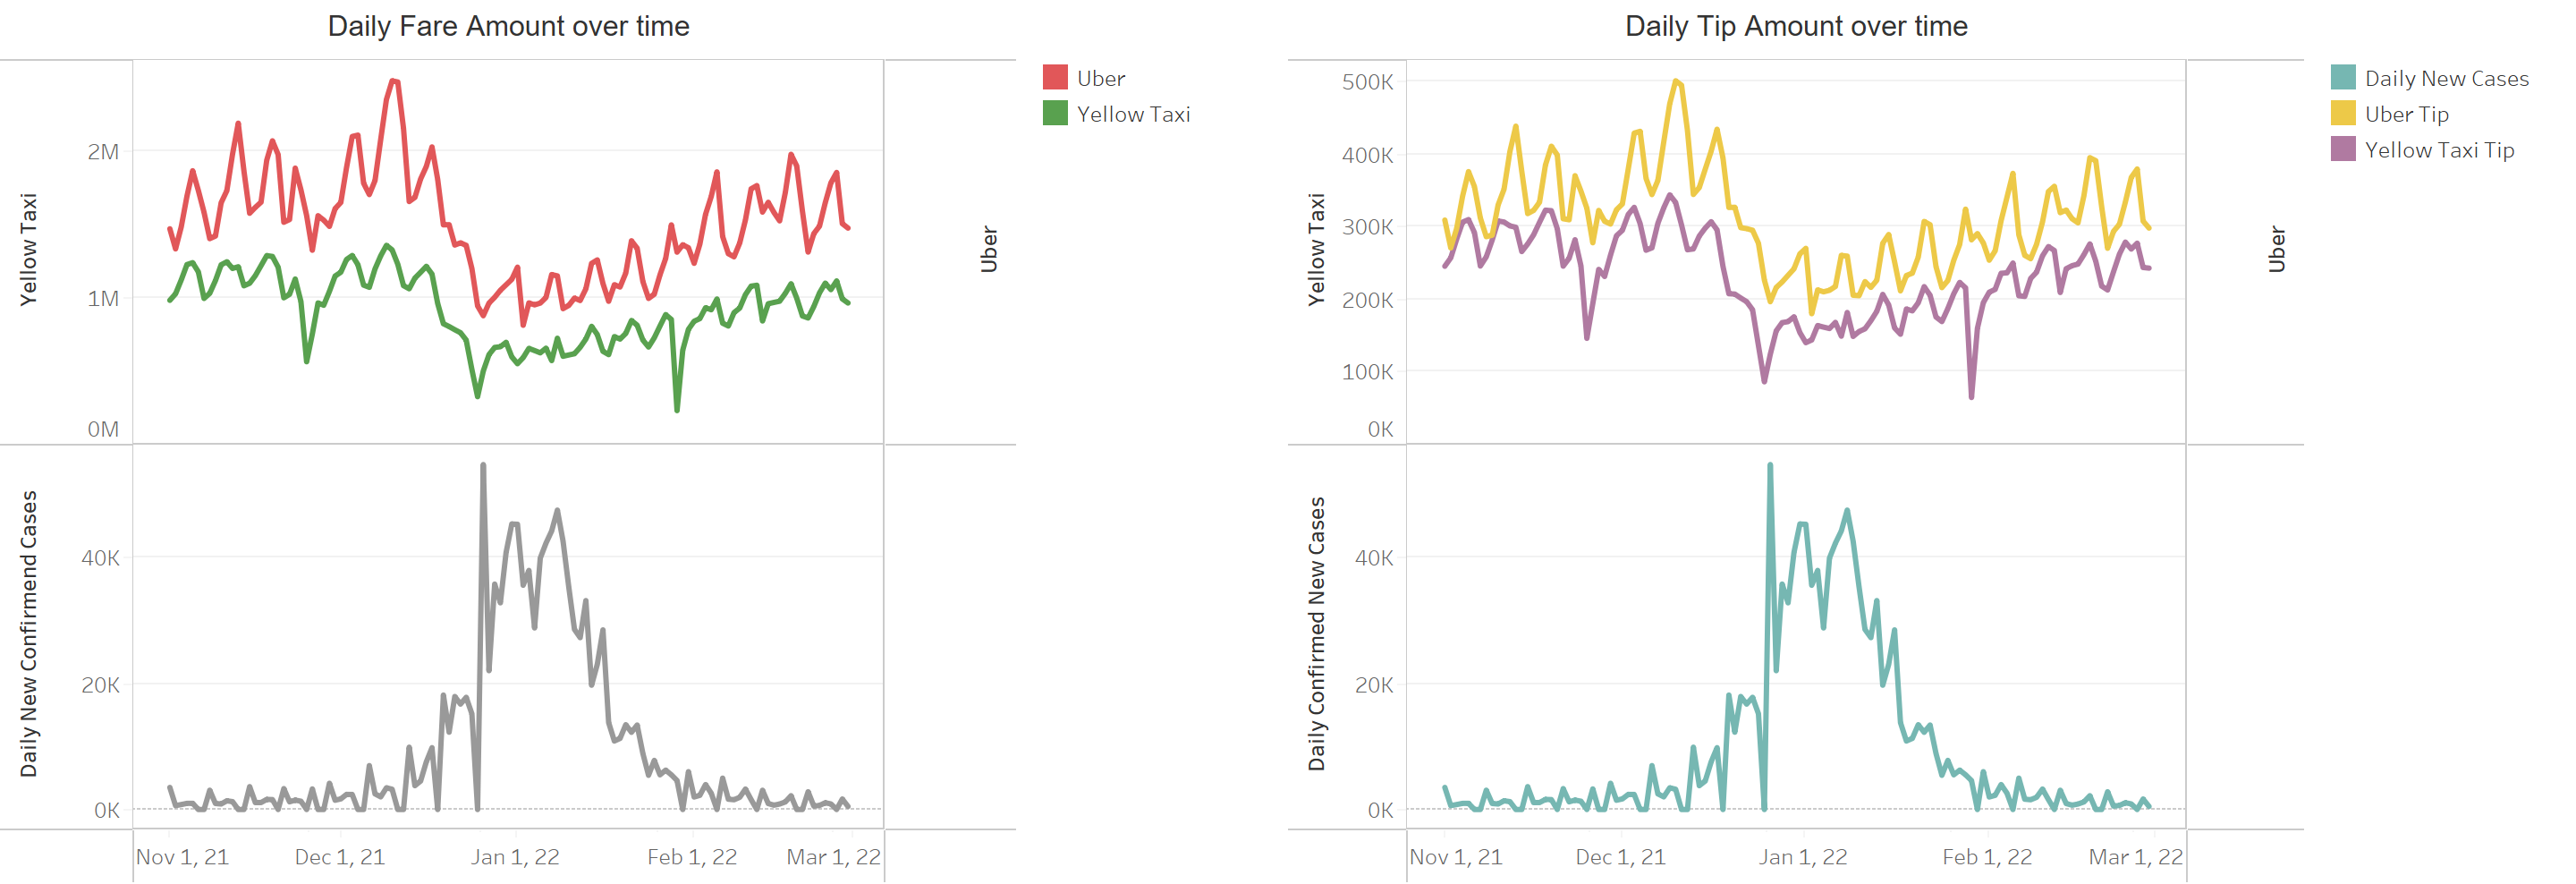
\includegraphics[scale = 0.18]{fare_and_tip_corona.png}
    \caption{Visualization of daily total fare/tip amount of yellow taxis and Uber and daily new confirmed cases over time.}
    \label{fig:coroa}
\end{figure}
Figure \ref{fig:coroa} visualizes the development of daily new confirmed cases in NYC. We can see that between late December and early January, there exists a peak of infections in NYC, where infections are doubled. In Figure  \ref{fig:coroa}, at the peak of infections, there exists a significant decrease in both fare and tip amount. It means that the outbreak of Covid-19 variants still hugely impacts transportation in NYC. And after the outbreak, riders pay less and tip less than pre-outbreak. 

\subsubsection{Yellow Taxi and Uber}
\begin{table}[]
    \centering
    \begin{tabular}{c|cc|cc}
    \hline
         Borough&  \multicolumn{2}{c}{Tip}& \multicolumn{2}{c}{Fare}\\ 
          \hline
         &Yellow Taxi& Uber&Yellow Taxi& Uber\\
         \hline
         EWR&0.00&0.54&0.00&2.56\\
         Queens&1.03&4.16&4.38&20.61\\
         Bronx&0.08&0.83&0.38&4.11\\
         Manhattan&10.99&9.11&42.75&42.55\\
         Staten Island&0.00&0.26&0.03&1.18\\
         Brooklyn&0.83&3.81&3.79&18.93\\
     \hline
    \end{tabular}
    \caption{Averaged tip/fare amount per trip in NYC boroughs.}
    \label{tab:tip}
\end{table}

From Figure \ref{fig:coroa}, before and after the outbreak of Covid-19 variants, Uber has a significant advantage over yellow taxi in terms of daily fare or tip amount. Table \ref{tab:tip} presents the averaged fare/tip amount per trip. We can see that passengers prefer to tip more and pay more for Uber drivers than for yellow taxis. Uber is not always cheaper than yellow taxis. From Table \ref{tab:tip}, Uber is at least twice more expensive than yellow taxis in NYC boroughs except for Manhattan in terms of average cost per trip.

\subsubsection{Boroughs}
\begin{figure}
    \centering
    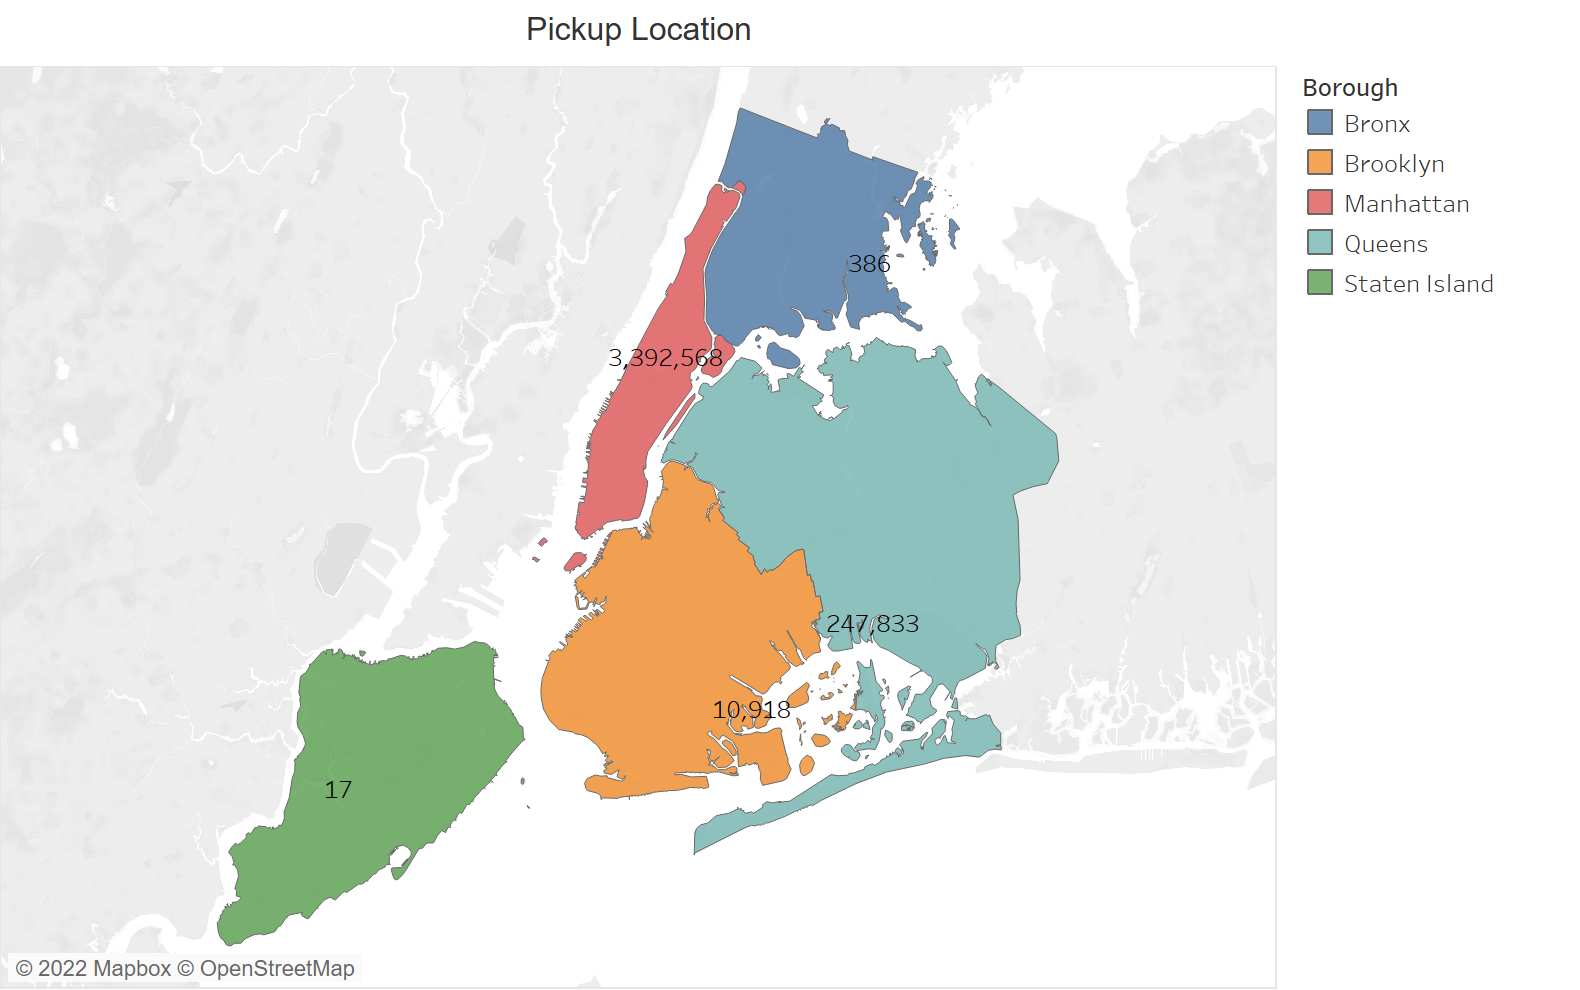
\includegraphics[scale = 0.25]{pickup.png}
    \caption{Averaged monthly pickup frequencies in NYC boroughs.}
    \label{fig:borough}
\end{figure}
Figure \ref{fig:borough} visualize averaged monthly pickup frequencies in five boroughs. Manhattan and Queens are the two most frequently visited of all boroughs. 
% You can have \section{}, \subsection{}, and \subsubsection{}

\section{Modelling}
We aim to predict the tip amount for a trip. We use instances from Nov 2021 to Jan 2022 to train the model and validate its performance. We use the trained model to predict the tip amounts on sampled instances in Feb 2022. 

\subsection{Feature Selection}
We measure the importance of features with mutual information. Mutual information of two random variables is a measure of the mutual dependence between the two variables \cite{mutual}. We select 10 features with highest scores given by mutual information, i.e. fare amount, trip time, trip distance, miscellaneous extras and surcharges, pickup and dropoff location, tolls amount, airport fee, rate code and passenger count.

\subsection{Models}
\paragraph{Linear Regression}
Linear regression fits a linear model with coefficients to minimize the residual sum of squares between the observed targets in the dataset, and the targets predicted by the linear approximation \cite{scikit-learn}.

\paragraph{Random Forest Regression}
A random forest is a meta estimator that fits a number of classifying decision trees on various sub-samples of the dataset and uses averaging to improve the predictive accuracy and control over-fitting
\cite{scikit-learn}. 


\subsection{Results}
We use Root Mean Square Error (RMSE) to measure the difference between predictions and actual values as described by Equation \ref{rmse}.  
\begin{align}
    RMSE = \sqrt{\frac{1}{n}\Sigma_{i=1}^{n}(Actual_i -Predicted_i)}
\label{rmse}
\end{align}

We randomly sample 40\% instances from each month between Nov 2021 and Jan 2022. 80\% of these instances made up train set. The rest builds the dev set. We randomly sample 60\% instances from Feb 2022 as the test set.
\begin{table}[]
    \centering
    \begin{tabular}{c|c|c}
    \hline
         Model& Dev Set & Test Set \\
    \hline
         Linear Regression& 1.59&1.52\\
         Random Forest (depth=2) & 1.59&1.52\\
         Random Forest (depth=4) & 1.50&1.42\\
         Random Forest (depth=6) & 1.48&1.42\\
         Random Forest (depth=8) & 1.48&1.42\\
    \hline
    \end{tabular}
    \caption{RMSE of linear regression and random forest models on dev and test sets}
    \label{tab:result}
\end{table}

\subsection{Analysis}
From Table \ref{tab:result}, we can see that the random forest model performs better than linear regression if we set a suitable value for the maximum depth of the tree. However, with the increase of the maximum depth, the random forest model overfits as the performance on the test set can not be improved any further. 


\section{Recommendations}
Yellow taxi has flatter pricing strategies than Uber. For instance, Taxis departing John F. Kennedy (JFK) International Airport charge a flat fare of \$52 for trips to Manhattan, plus any tolls and tips \cite{benefit}. In contrast, Uber has canceled the flat fare option, which may cause 2-3 times high fares than with taxis for passengers. We recommend that yellow taxis can customize some trips that include frequently visited locations, such as a trip between Manhattan and JFK airports. Because Manhattan is the most commonly visited by riders among the five NYC boroughs, and for these customized trips, yellow taxis offer a flat price. 

However, price is not the only factor that affects user decisions. According to our analysis, Uber does not have much price advantage over yellow taxis. From the tip amount, we can infer that riders are probably more satisfied with the service provided by Uber drivers. We recommend that riders can score for the service of drivers. If a yellow taxi driver has enough scores, he can have a medallion on his car. However, this medallion will be removed if scores become lower than a threshold. For longer trips, newcomers, and passengers with high income, we believe that taxis with medallions are more reliable and thus better options for them.


\section{Conclusion}
We explore the factors that influence the riders using yellow taxis. The outbreak of Covid-19 still has an unignorable impact on the rider's decision-making. Up to now, 78\% of NYC residents are fully vaccinated. We hope that the high vaccination rate can contribute to economic recovery. Uber dominates in the land of the classic yellow taxi. We hope that yellow cab can optimize its pricing strategies and services. 

On March 24th, 2022, Uber announces its cooperation with yellow taxis in NYC. It means that on the Uber app, passengers will find Yellow taxis as their driving options. Yellow taxis are expected to attract more riders through this platform.



\clearpage

% BEGIN REFERENCES SECTION
\printbibliography

\end{document} 


  